\documentclass[8pt]{article}
\usepackage[spanish]{babel}
\usepackage[utf8]{inputenc}
\usepackage{titlesec}
\usepackage{hyperref}
\usepackage{graphicx}
\graphicspath{ {/} } 


\usepackage{vmargin}
\setpapersize{A4}
\setmargins{1.5cm}       % margen izquierdo
{1.5cm}                        % margen superior
{16.5cm}                      % anchura del texto
{23.42cm}                    % altura del texto
{10pt}                           % altura de los encabezados
{1cm}                           % espacio entre el texto y los encabezados
{0pt}                             % altura del pie de página
{2cm}                   



\titleformat{\bfseries}

\title{ Aceleración de los procesos de inversión en RH sobre perfiles fotosféricos.}
\date{31 March, 2019}
\author{Ferran Domingo García}


\begin{document}

	\maketitle
	\newpage

	\tableofcontents
	\newpage

	\begin{abstract}
	
		Este trabajo pretende presentar una forma nueva de acelerar los procesos de inversión llevados acabo hasta hora de forma iterativa para solución de la ecuación de transporte radiativo mediante el uso de redes neuronales de profundidad variable. El grueso del trabajo se centra la implementación y estudio de la eficiencia dichos módulos, cuya fuente de código queda en manos de la comunidad científica para su posterior uso. El marco de trabajo de la red se basa en el los perfiles sintéticos generados con programa en IDL y Fortran: DESIRE, propiedad de Basilio Ruiz (IAC), que ha puesto a mi disposición. \newline
		
		Este trabajo constituye un análisis riguroso de la eficiencia de dicho código, en que se discute detalladamente las bases físicas del programa de síntesis de espectros, y como las estructuras DNC se pueden integrar de forma orgánica al reconocimiento, identificación y clasificación de ....  \newline
		
		Como aplicación más directa del estudio, animo a la comunidad a integrar dichas rutinas sobre los sistemas adquisición para la clasificación de observaciones potencialmente interesantes, ya sea para identificar casos anómalos, como para acelerar el proceso de inversión de y de este modo economizar tiempo y recursos. Espero que ello suponga un precedente en la nueva generación de telescopios solares, lo que potencialmente vendría solucionando un escenario en donde nuestra capacidad de procesado de observaciones resulta insuficiente para un flujo de datos renovado, que ...........
		
	\end{abstract}\newpage
	
	\renewcommand\abstractname{Agradecimientos}
	
	\begin{abstract}
		
		Agradezco altamente a Basio Ruíz y Andrés Asensio, mis colaboradores, su ayuda y asesoramiento en el proceso de desarrollo del trabajo, como su inestimable amabilidad a la hora de prestarme apoyo por teleconferencia cuando esto fue necesario debido a la difícil situación vivida durante el estado de alerta del COVID-19. También me gustaría destacar la comprensión por la situación personal en la que me encontré a la hora de escribir y realizar el trabajo que aquí os presento, y por la que estoy altamente agradecido.	\newline
		
		También agradezco a la comunidad de programadores y investigadores, que de forma continuada comparten, de forma desinteresada, conocimientos y apoyo técnico sobre plataformas web, como GitHub, sin las que mi trabajo habría resultado mucho más duro.\newline
		
		De esta forma pretendo contribuir dejando aquí un repositorio del código fuente, abierto a que quien lo necesite, para que pueda reciclarlo o actualizarlo :\newline
		
		\url{https://github.com/fedogar/Neural_RH_Inversion}
		
	\end{abstract}\newpage
	

	\section{Introducción}

	Durante la última mitad del siglo XX los procesos de cálculo numérico han ayudado a evidenciar y refutar las bases de los conocimientos teóricos recopilados durante más de 3 siglos. Puede decirse que desde los inicios siglo XVIII la parte experimental de la ciencia constituye uno de los pilares básicos del método científico. Hoy, desde la entrada en el siglo XXI y el avance de las tecnologías, los escenarios físicos que podemos tratar se extienden de forma cada vez más del espacio físico donde podemos realizar nuestros experimentos. Esto, ha hecho que sea posible simular de forma numérica procesos físicos que ocurren en lugares donde actualmente no es posible realizar mediciones, pero que conceptualmente resulta aún más ambicioso ya que permite tratar escenarios hipotéticos, y contrastar resultados con un grado de sensibilidad que cada vez más, supera a la de nuestra instrumentación experimental.\newline
				
	Como escenario arquetipo donde la simulación numérica resulta beneficiosa para un físico, encontramos el campo de la astrofísica, por motivos obvios. En particular resulta beneficioso, en procesos que involucran una cantidad elevada de datos donde el estado del arte de nuestra tecnología puede dar su máximo rendimiento.********************************** \newline
	
	Este artículo se ve precisamente motivado en el proceso de adaptación tecnológica a nuestra forma de hacer ciencia.\newline
		
	Este trabajo aparece articulado en dos bloques conceptuales diferentes, por lo que en todo momento se hará énfasis si nos encontramos en la discusión de la parte física del problema o un análisis sobre los aspectos relacionados con el programa de simulación numérica. La estructura que se ha seguido es la siguiente:\newline
	
	
	\subsection{Introducción teórica y metodológica}
	
	Como primer objetivo, el trabajo pretende asentar las bases del \emph{cálculo de inversión}, de forma que quede clara la metodología de cálculo, los distintos aspectos importantes en implementación para el código de síntesis, y las bases físicas en las que se sustenta el fenómeno, con especial énfasis en el número de parámetros empleados y su dependencia funcional, y de que manera el uso de redes neuronales puede agilizar el proceso de cálculo.\newline
	
	 Para introducir las bases físicas del cálculo de inversión, expondremos brevemente las bases del de lo que es la ecuación de transporte radioativo y la importancia/utilidad de emplear un tratamiento en base a parámetros de Stokes en lugar del habitual formalismo matricial de Jones, los cuales discutiremos. A continuación, trataremos bajo que suposiciones y restricciones trataremos los modelos de atmósfera solar con los que trabajaremos, de manera que quede acotado el régimen de validez de los resultados expuestos en secciones posteriores.\newline
	 
	 *********Atómica??
	
	Una vez expuesta la implementación en el estado del arte del proceso de inversión, con la que he tenido la suerte de poder trabajar, exploraremos el método síntesis a través de redes neuronales, discutiendo aspectos técnicos sobre como preparar los datos y su posterior reconstrucción.\newline
	
	Debido a que este artículo no asume conocimientos avanzados previos en la estructura de redes neuronales**, discutiremos los aspectos más importantes . En el trabajo se exploran distintos tipos de estructuras, al igual que el uso de distintos optimizadores, atacaremos dichos conceptos y las ventajas que aporta el empleo de unas u otras, de manera que queden ejemplificados al aplicarlo a nuestros modelos sintéticos.\newline
	
	Ejemplos de la implementación de los distintos programas, pueden consultarse en el repositorio \url{https://github.com/fedogar/Neural_RH_Inversion}. De manera que nombraré y describiré brevemente cada parte empleada para obtener cada resultado, pero dejando los detalles más técnicos sobre como se implementan los algoritmos el repositorio, con la regla de hacer referencias a pie de página con comentarios que faciliten la comprensión del repositorio cuando resulte oportuno.
	
	
	
	\subsection{Introducción sobre resultados y conclusiones}
	
	La estructura en que se presenta el análisis de resultados simulados se divide en 5 bloques.\newline
	
	Los dos primeros de ellos corresponden a los resultados previos al método de inversión, en los que se ha implementado una primera red que interpola los valores de profundidad, temperatura y presión gaseosas a sus equivalentes en profundidades ópticas, lo que permite entrar en una primera fase donde aceleraremos un proceso de integración numérica. En este bloque también englobamos el proceso de síntesis de espectros a partir de cubos de datos que contienen los parámetros físicos de la estructura de la atmósfera solar, con dependencia de las profundidades ópticas, para un conjunto de líneas espectrales de interés\footnote{Dejamos el modelo de transiciones atómicas empleado en el cálculo como anexo, que puede ser consultado}.\newline
		
	El segundo y tercer bloque ataca el problema inverso, dados los perfiles sobre un conjunto de lineas espectrales obtendremos los parámetros físicos en función de la profundidad óptica. Discutiremos el grado de sensibilidad de los resultados y acotaremos el régimen en el que podemos confiar en nuestro método de inversión, con los datos proporcionados por el IAC\footnote{Basilio Ruiz Cobo, Enero 2020 - simulación Bifrost},  lo que se conoce en la jerga como \textit{overfitting} y \textit{underfitting} de los métodos ML. Reservamos un apartado especifico a lo que són la inserción de perfiles atípicos, o que caen fuera del set de entrenamiento de la red, y como establecer un proceso de clasificación de las observaciones. Para este proceso de simulación emplearemos dos hipótesis en el proceso de simulación: NLTE y LTE**** \newline 
	
	Para terminar resumiremos los resultados obtenidos, extrayendo conclusiones y posibles vías de aplicación futuras a las RNN sobre el campo, extendiendo el problema NLTE.	
	
		
		\section{Base teórica}
		
			\subsection{Ecuación de transporte radioativo}
				
				\subsubsection{LTE}
				
				\subsubsection{NLTE}
		
		\subsection{Perfiles espectrales}
		
			\subsubsection{Formalismo de Stokes}
			
			\subsubsection{Modelos atómicos}

		\subsection{Modelos solares}
		
		
		\subsection{Estado del arte}
		
			\subsubsection{Síntesis espectral}
		
			\subsubsection{Proceso de inversión en RH}
	
		\subsection{Ml: RNN}
		
			\subsubsection{Redes lineales: RNN}
			
			\subsubsection{Redes convolucionales}
			
			\subsubsection{******}
			
		\subsection{Hipótesis sobre los modelos}
		
		Principalmente aparecen dos bases de suposiciones fundamentales que facilitan o no el cálculo de la ecuación de transporte ...
	
	
		\section{Simulación numérica - Entrenamiento Z : LOG(Tau)}
		
		
		
		
		Los datos que mostramos acontinuación provienen de la simulación Bifrost: Marzo 2020 - Proporcionados por Basilio Ruiz - IAC 2020.\newline
		
		Tras una primera fase visualización del set de pixeles, gráfica X, observamos que esta constituye un ejemplo claro de la necesidad de tratar el set antes de entrenar la red\footnote{Claramente este caso solo sirve como pretexto para remarcar la importancia  una buena calidad de datos, necesaria para la convergencia de cualquier red neuronal, lo que permite generalizar , y garantizar precisión en la solución al problema} , ya que se observa poco contraste entre estructuras lo que hace intuir la aparición de data dañada.\newline
		
				\center \includegraphics[scale=0.4]{Presure-}
		
		
		El criterio empleado para aislar los pixeles corruptos tras una primera visualización, fue identificar los datos comprendidos en los percentiles del 0.005 y 99.995 y substituirlos por un pixel central del cubo de datos. Tras el proceso de filtrado 	mostramos el mismo set de gráficas a continuación.	


		\center 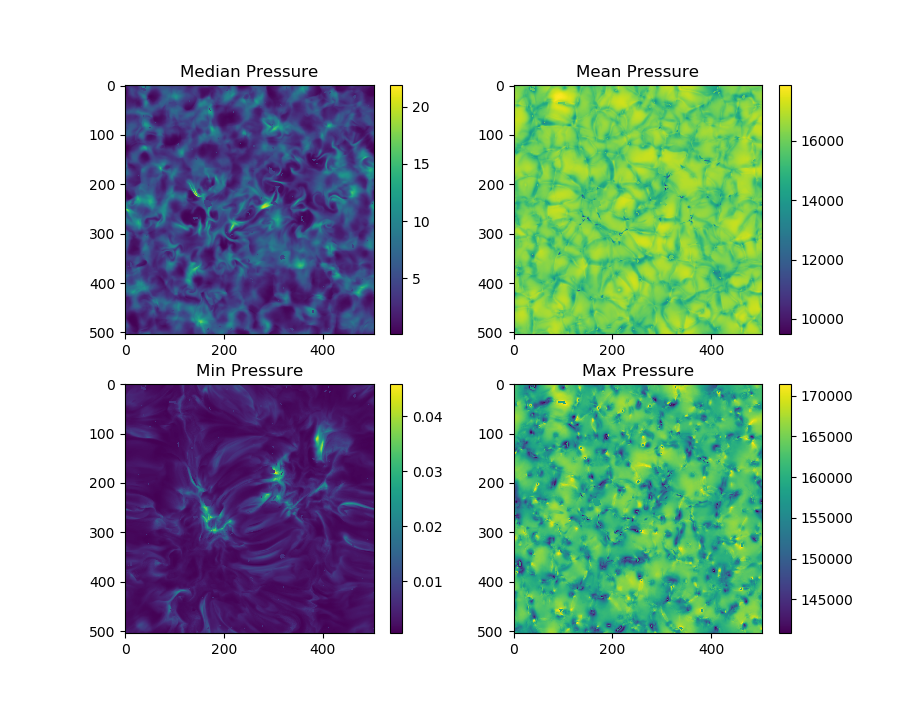
\includegraphics[scale=0.5]{Pressure-Z-OK.png}
		
		
		Las gráficas *** permiten interpretar la estructura interna del modelo solar: de manera que los mínimos de temperatura corresponden a la estructura de las capas altas de la fotosfera, donde se observa un régimen altamente convectivo, caracterizado por estructuras toroidales si atendemos a los mínimos de presión, que revelan la estructura magética en dicha capa. Por el contrario, sobre los máximos de presión observamos lo que es la estructura granular de la cromosfera, que más claramente se vere reflejada en la gráfica Y:  
				
		\center 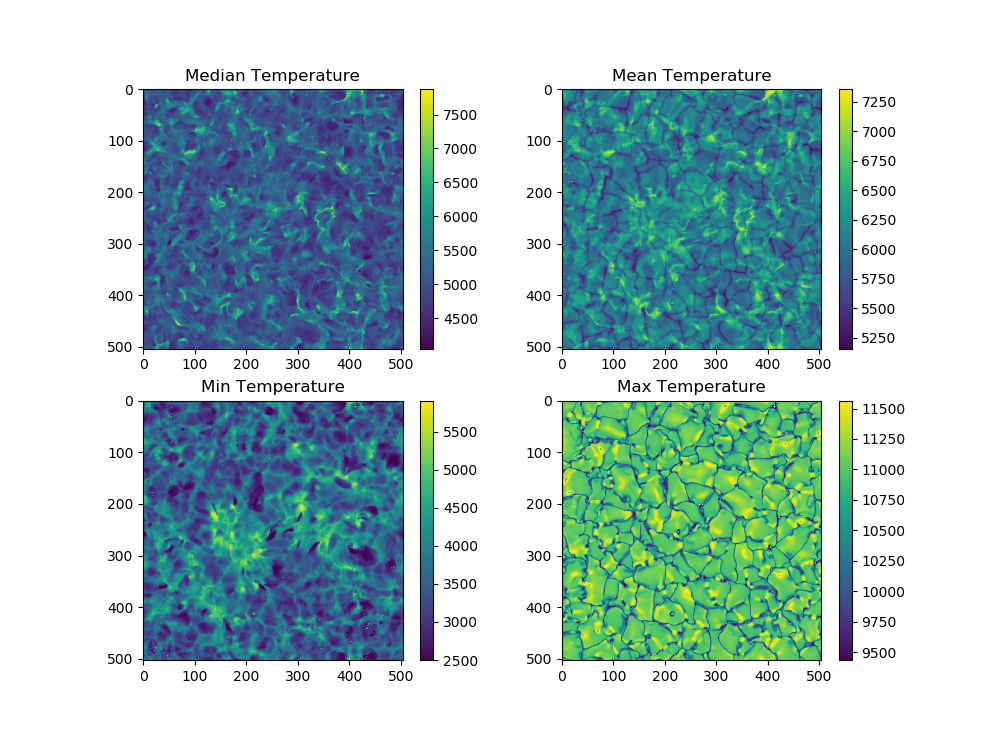
\includegraphics[scale=0.5]{Temperature-OK.png}		
				
		Las primeras imágenes corresponden a el estado de la atmósfera en la escala de profundidades 
		Z usual, de 161 valores que con los que iterativamente mediante integración numérica calculamos sus equivalentes en profundidades ópticas (equiespaciados)\footnote{Debido a las restricciones del sofwear facilitado (DESIRE : Basilio Ruiz &Co), el mero hecho de la necesidad de un equiespaciado para la síntesis de perfiles espectrales, nos obliga a interpolar los valores de otras variables, como presión y Temperatura, de manera que el uso de redes no solo si no que }, géficas X,Y.\newline
		
		
		 Los valores de las demás variables en profundidades se deben entender como una interpolación sobre los Z correspondientes a la escala de logarítmica de profundiades ópticas. Debido a detalles técnicos, de utilidad, nos restingiremos a una escala de profundiades ópticas de 86 niveles, en lugar de una conversión del los 161 en la escala usual, la razón será que para la síntesis espectral, los fotones que se generan en capas realmente profundas del modelo solar, debido al alto grado de compactación(alta densidad) del medio cuentan con un recorrido libre medio despreciable en el core, por lo que establecemos una cota (sobre 2 en logaritmos de profundidades ópticas) donde de forma efectiva comienzan a poder sintetizarse las primeras líneas que escapan a la atmósfera. \newline
		
		\center 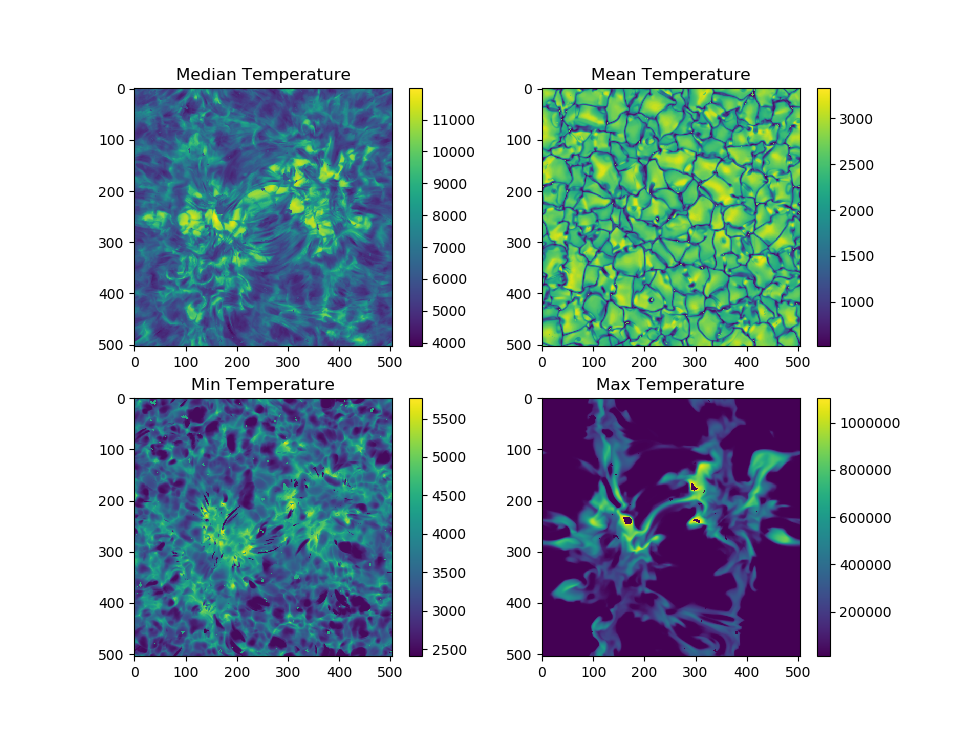
\includegraphics[scale=0.5]{Temperature-Tau-Ok.png}		
		
		Las gráficas X, Y muestran una estructura diferenciada si nos limitamos a los mínimos y máximos de presión electrónica y temperatura, respecto a las gráficas en escala de profundidades habitual. Como era de esperar, la presencia de la granulación es más marcada en el uso de presión electrónica a presión gaseosa, ya que nos encontramos en capas más profundas con temperaturas mayores, donde el grado de ionización supera las proporciones de átomos neutros, lo que facilita ver el contraste entre interfase en los gránulos. En la nueva escala, por motivos obvios, aparece una contribución mayor de las capas densas a los valores medios\footnote{Es debido a que en la escala habitual, una mismo recorrido de integración (Z) contribuye mucho menos a un incremento de la profundidad óptica, que en lugares donde el recorrido libre medio es menor, que usualmente es función casi exclusivo de la densidad.}. 		
		
		\center 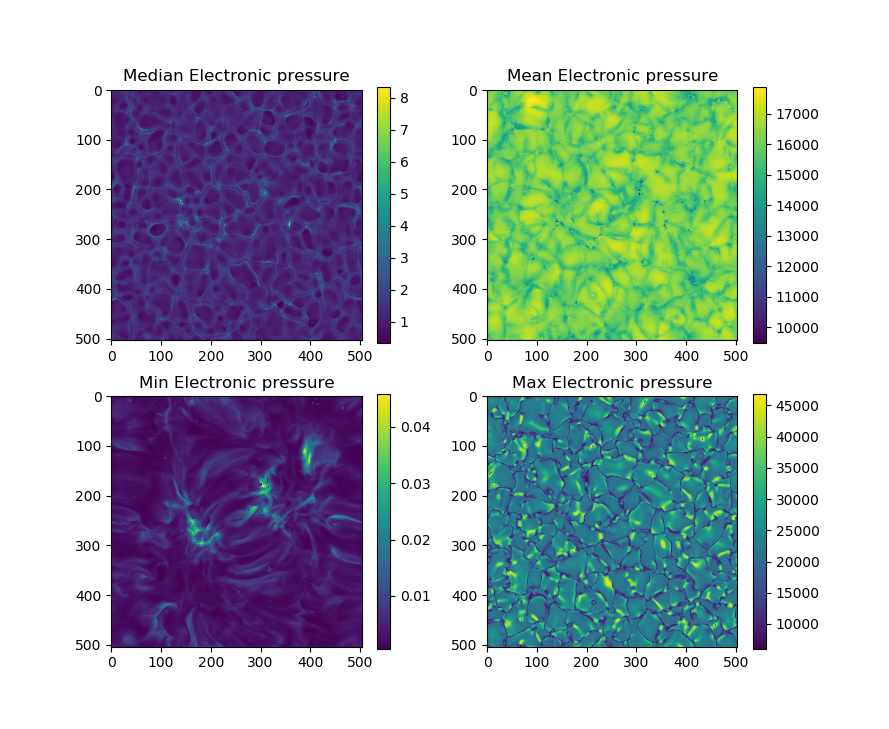
\includegraphics[scale=0.5]{Pressure-OK.png}		
		
		
			

	 
	   
		En un segundo estadio normalizamos las variables del set, de forma que trabajamos con valores adimensionales con de poco espacio de memória requerido, y que facilita las operaciones lógicas de la CPU. El criterio establecido fue tomar un valor típico, basado en la media del conjunto, aunque podría haberse tomado otro valor elegido de forma independiente localizado a una profundidad media para cada variable. \newline
		
		El hecho de emplear la un valor medio de las variable, pretende garantizar la eficiencia para cubos donde aparece un cambio de varios ordenes de magnitud entre el máximo y mínimo de cada variables, de manera que por su definición, la media (y no la mediana), se sitúa más próxima valores a los valores máximos. Procediendo de esta manera, lo que se garantiza es que todas las variables tras la normalización se encuentren en el rango de [0,100] aproximadamente, en valor absoluto.\newline

		Los resultados del entrenamiento son ...
		
		
			\subsection{Suposiciones}
			
			\subsection{Modelos}
			
				
			
	
		\section{Resultados y Conclusiones}
		
		\subsection{Resultados síntesis espectral}

		\subsection{Resultados inversión}
		
		\subsection{Régimen de validez y valores atípicos}
			
		\subsection{Conclusiones}



\end{document}
